
\subsection{Test Plan Objectives}
This document describes the testing done on the patient handling software produced by HeartByte for our customer Region Östergötland. This document will map the testing procedure as a whole and provide information to how the tests are selected, created and executed. There will also be definitions of what requirements the tests are made to ensure aswell as environment setup and tools used to ensure proper testing. This testplan will follow the structure provided by guru99 [1]. This is a living document which means that it will be updated over time to meet the current requirements.

\subsection{Scope}
\subsubsection{In Scope}

\begin{itemize}
  \item Functional Requirements
\end{itemize}
  These are placeholder pictures, they look bad but will change as new SRS is updated. To see better version of req go to either SRS or the General / analysis / requirements.xlsx

  \vfill
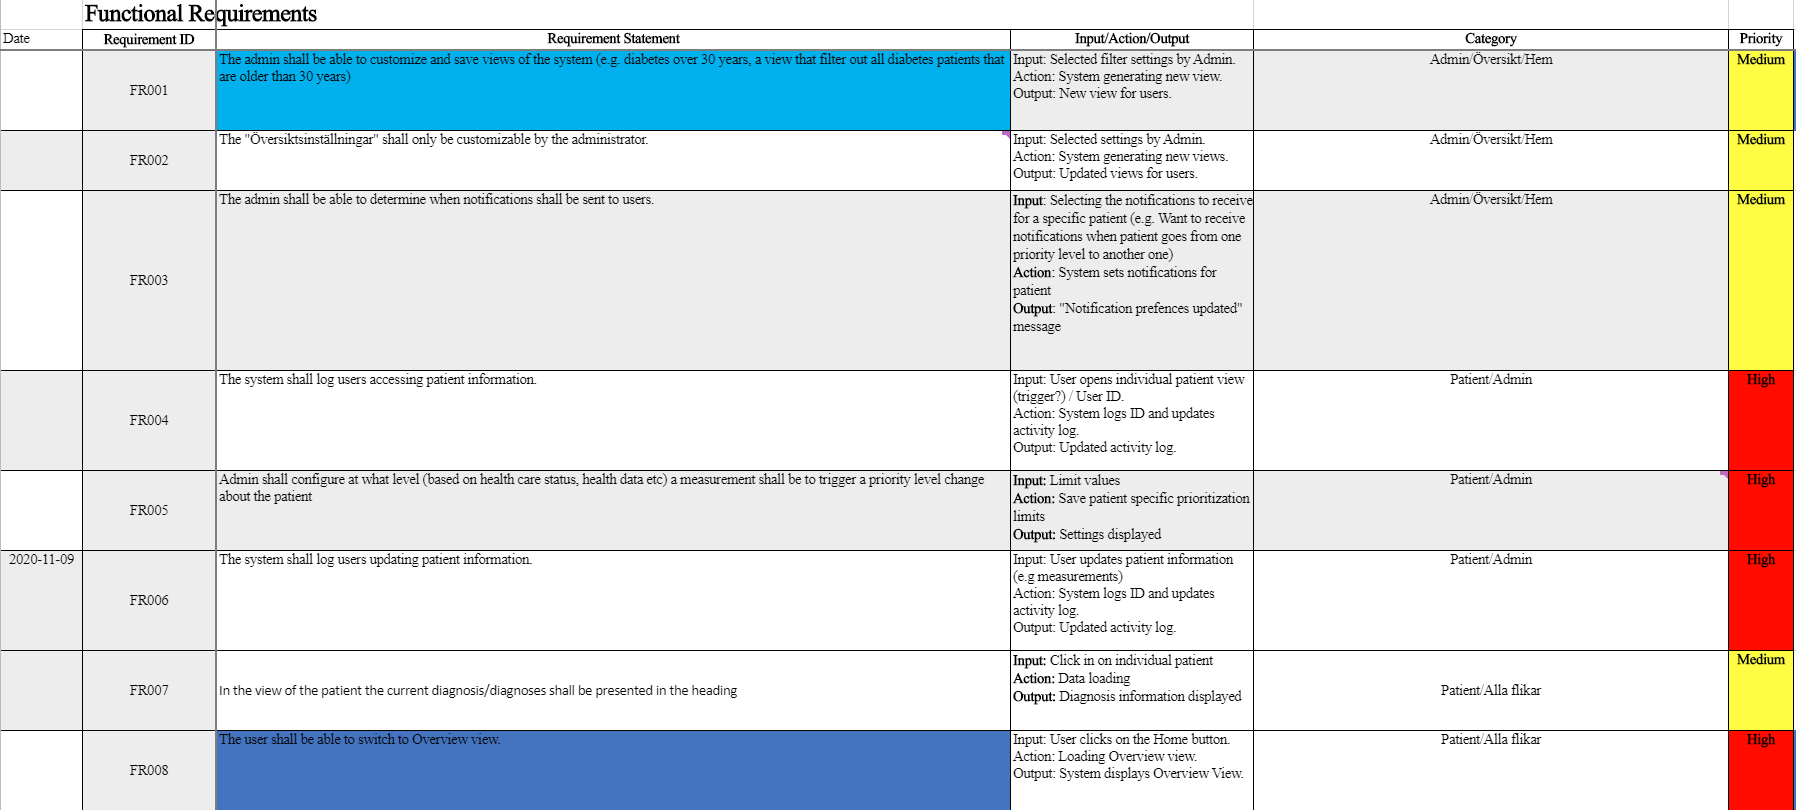
\includegraphics[width=\linewidth]{Pictures/Func1} (1)

    \vfill
    \vfill
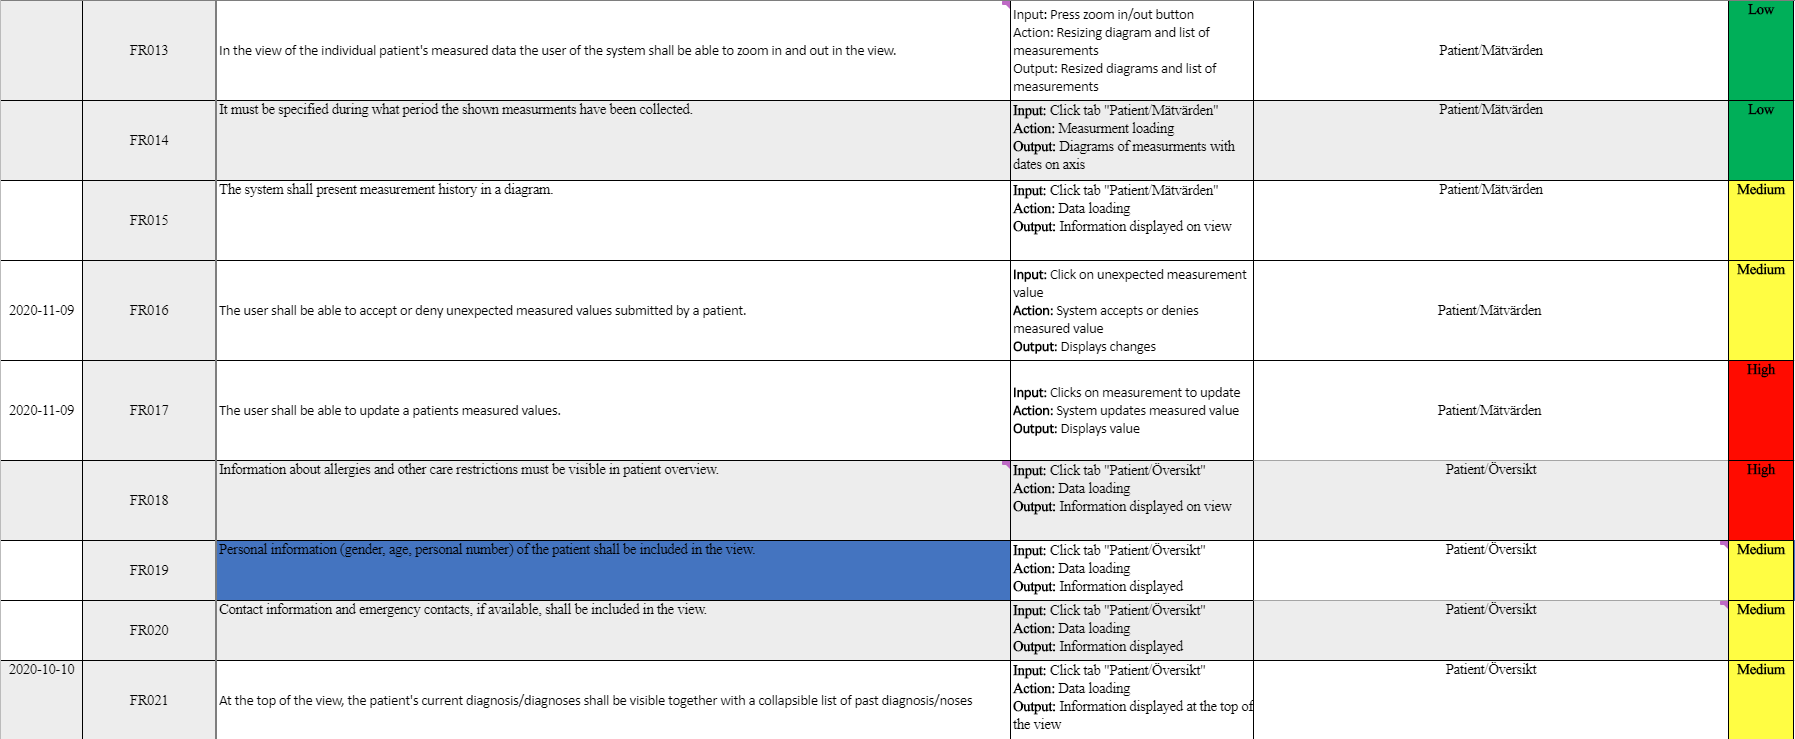
\includegraphics[width=\linewidth]{Pictures/Func2} (2)

    \vfill
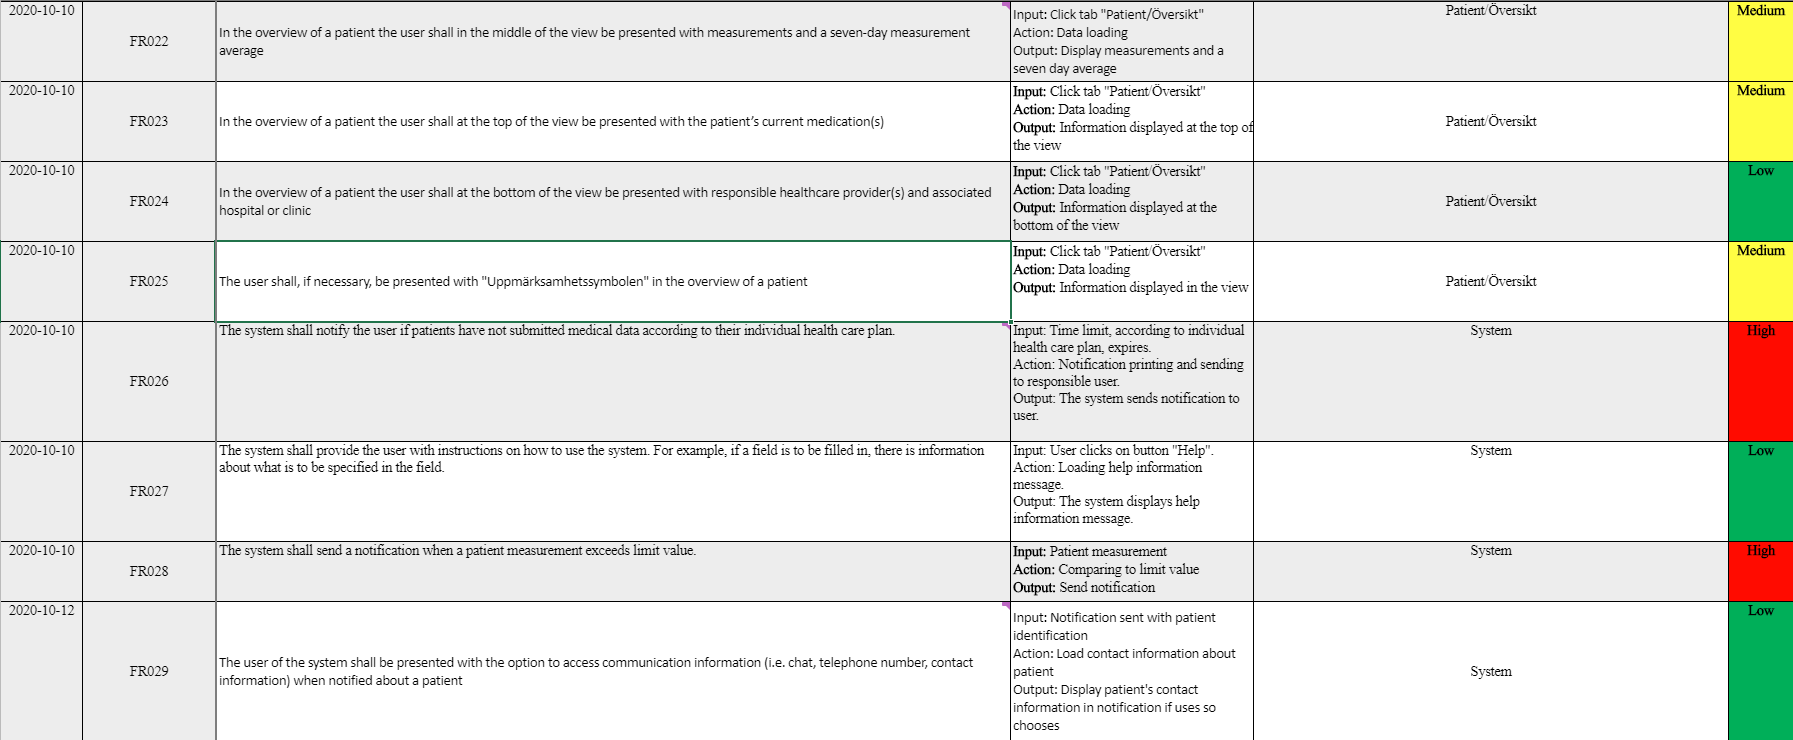
\includegraphics[width=\linewidth]{Pictures/Func3.PNG} (3)

    \vfill
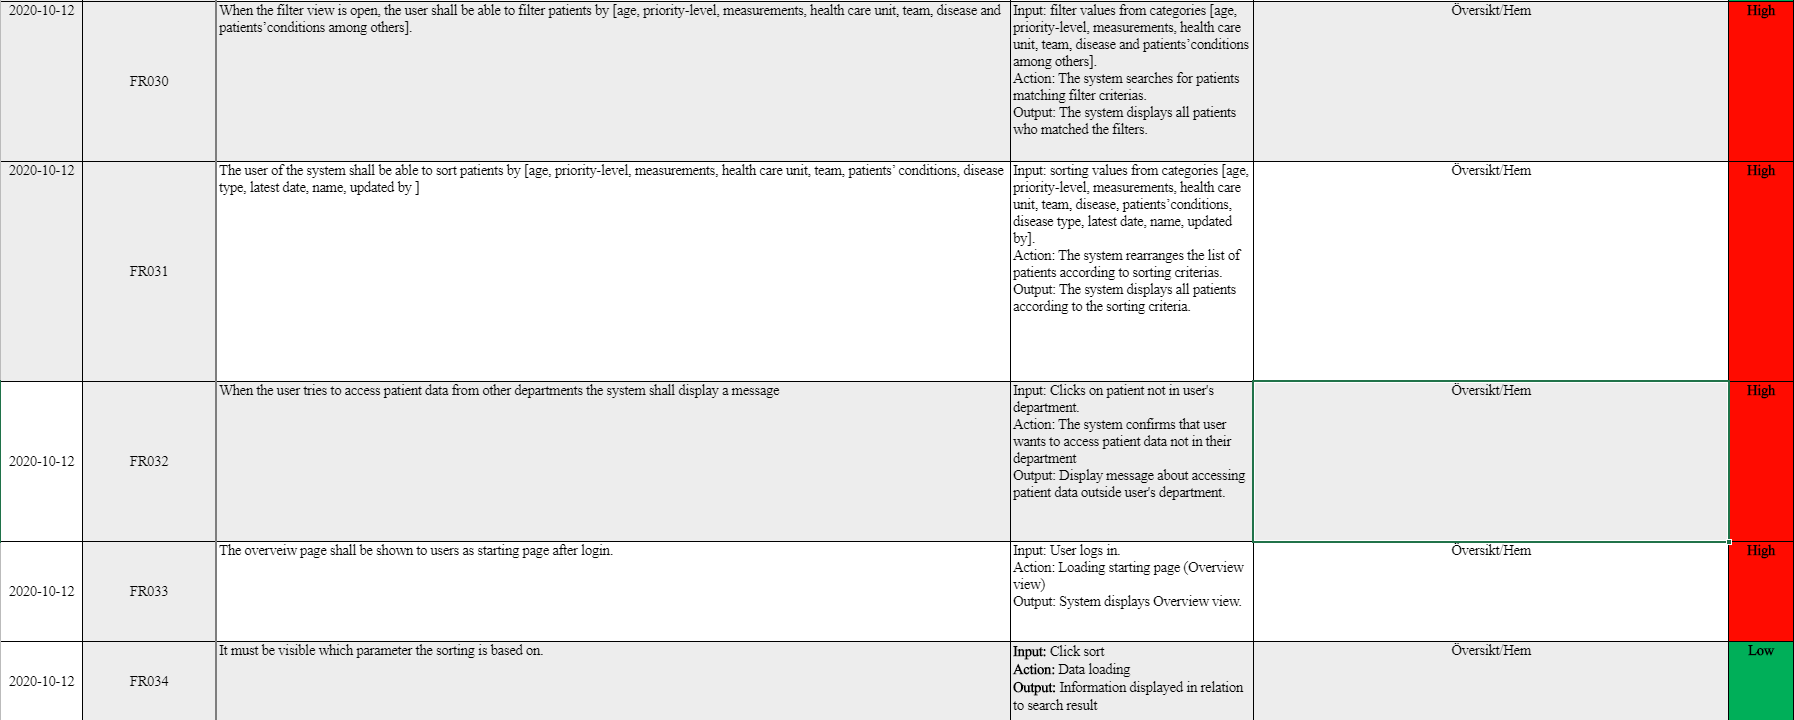
\includegraphics[width=\linewidth]{Pictures/Func4} (4)

    \vfill
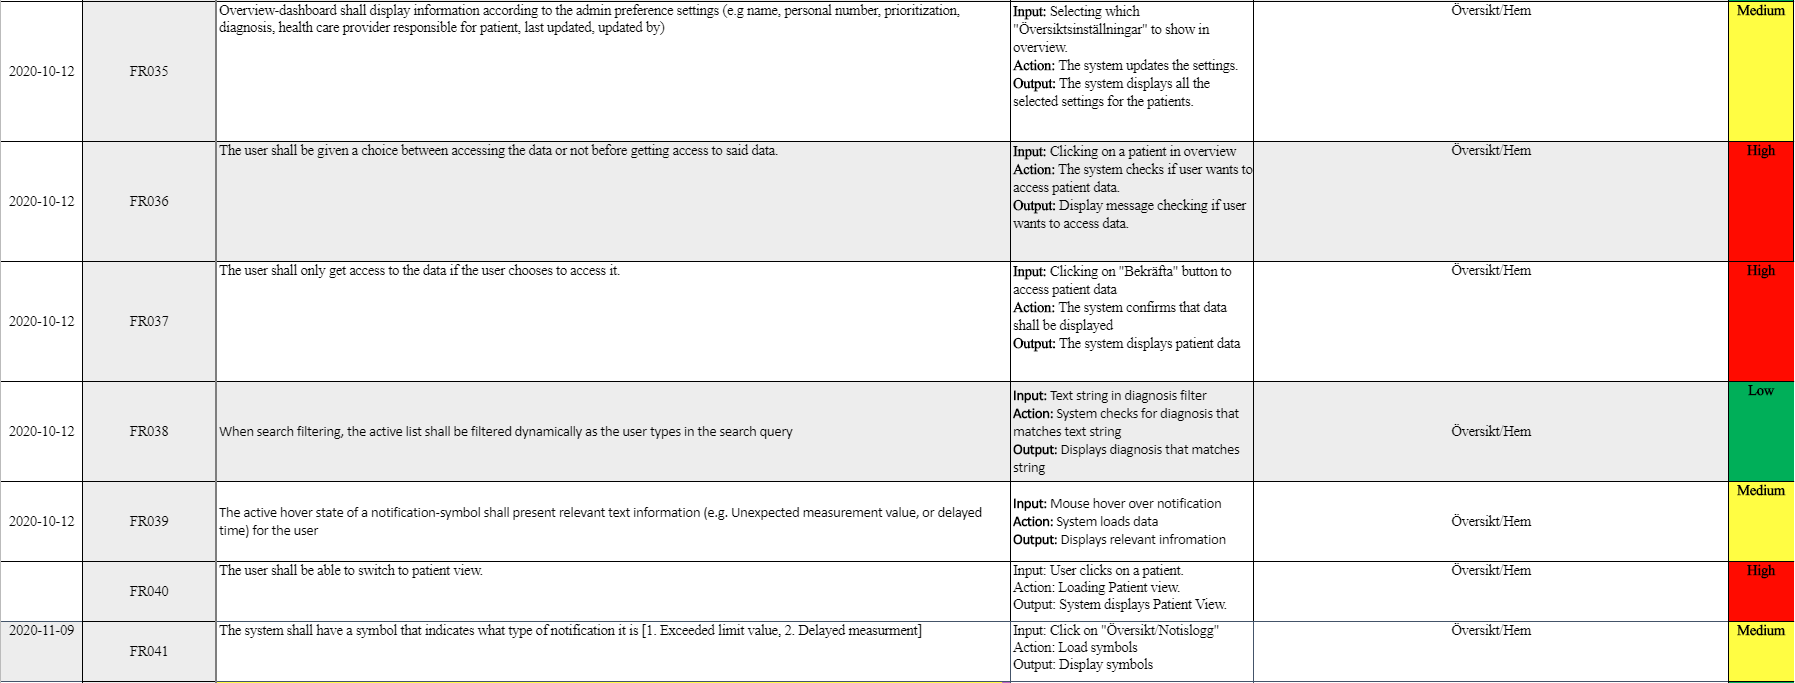
\includegraphics[width=\linewidth]{Pictures/Func5} (5)

    \vfill
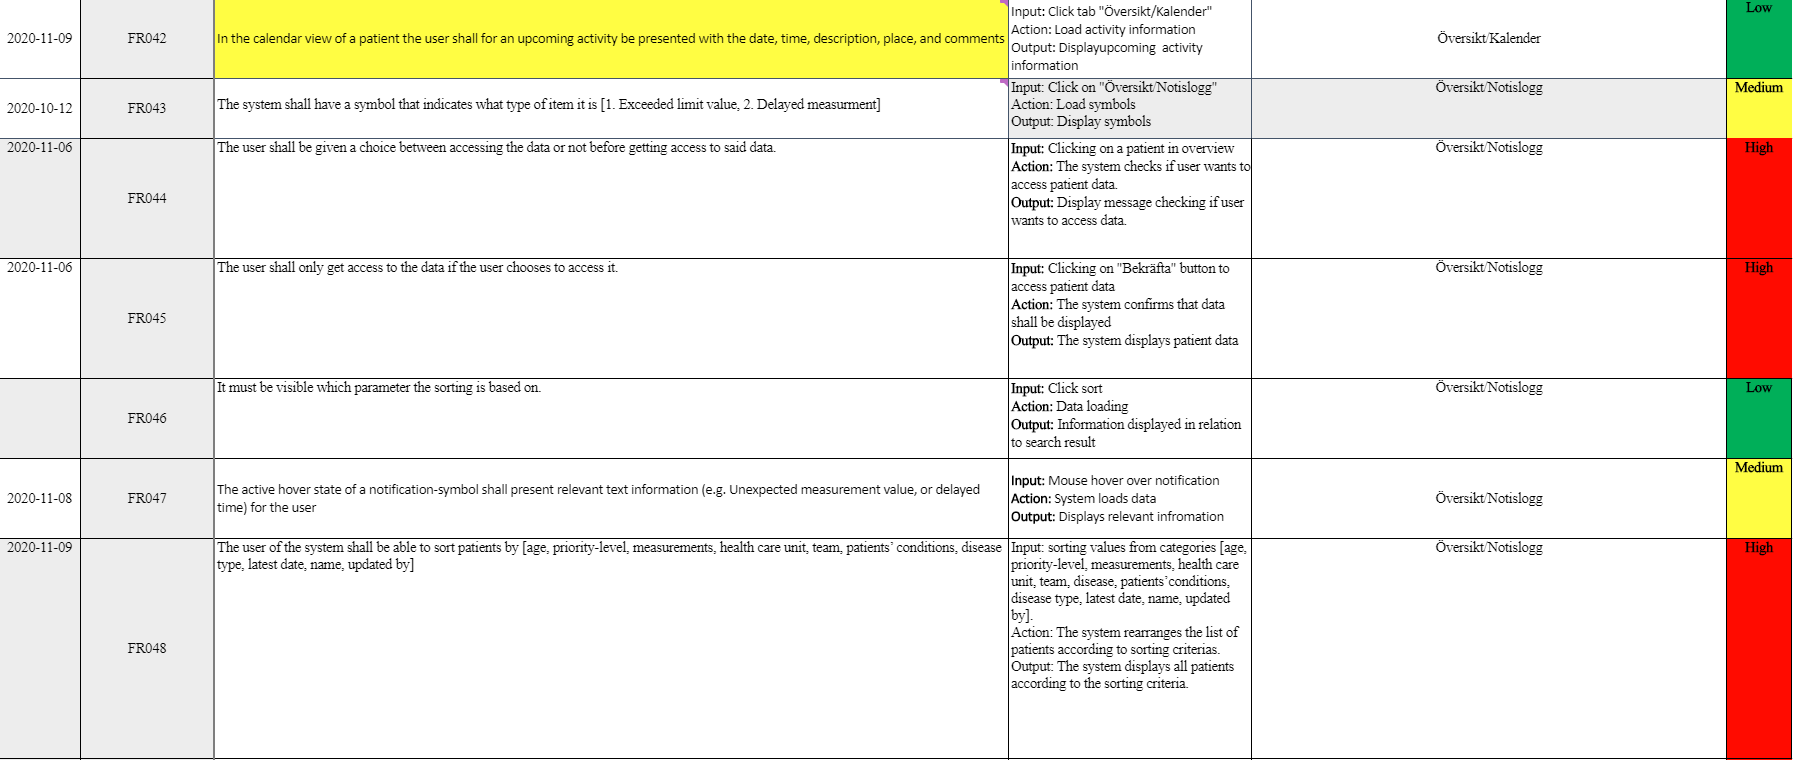
\includegraphics[width=\linewidth]{Pictures/Func6} (6)

    \vfill
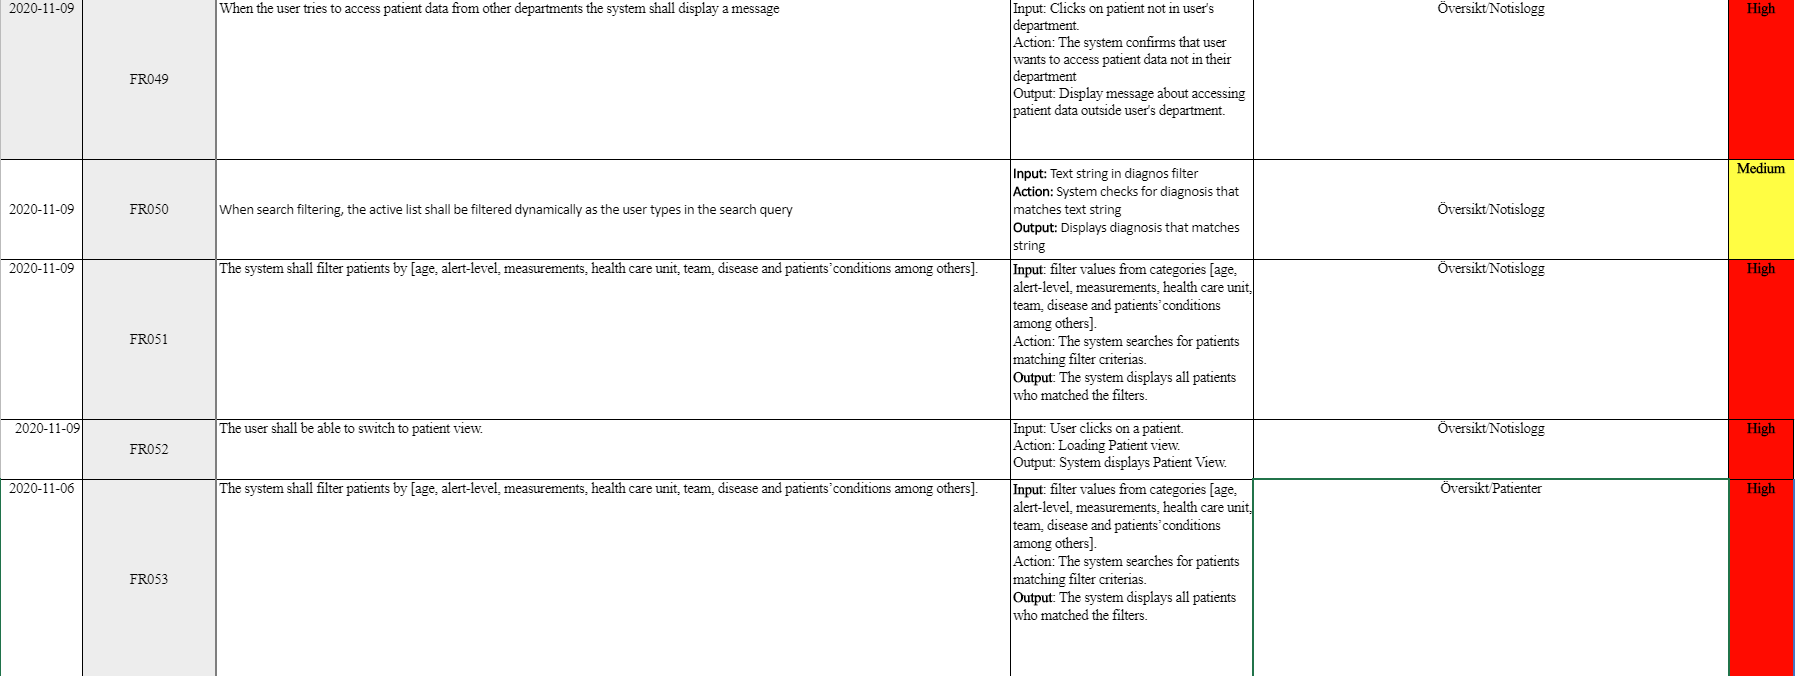
\includegraphics[width=\linewidth]{Pictures/Func7} (7)

    \vfill
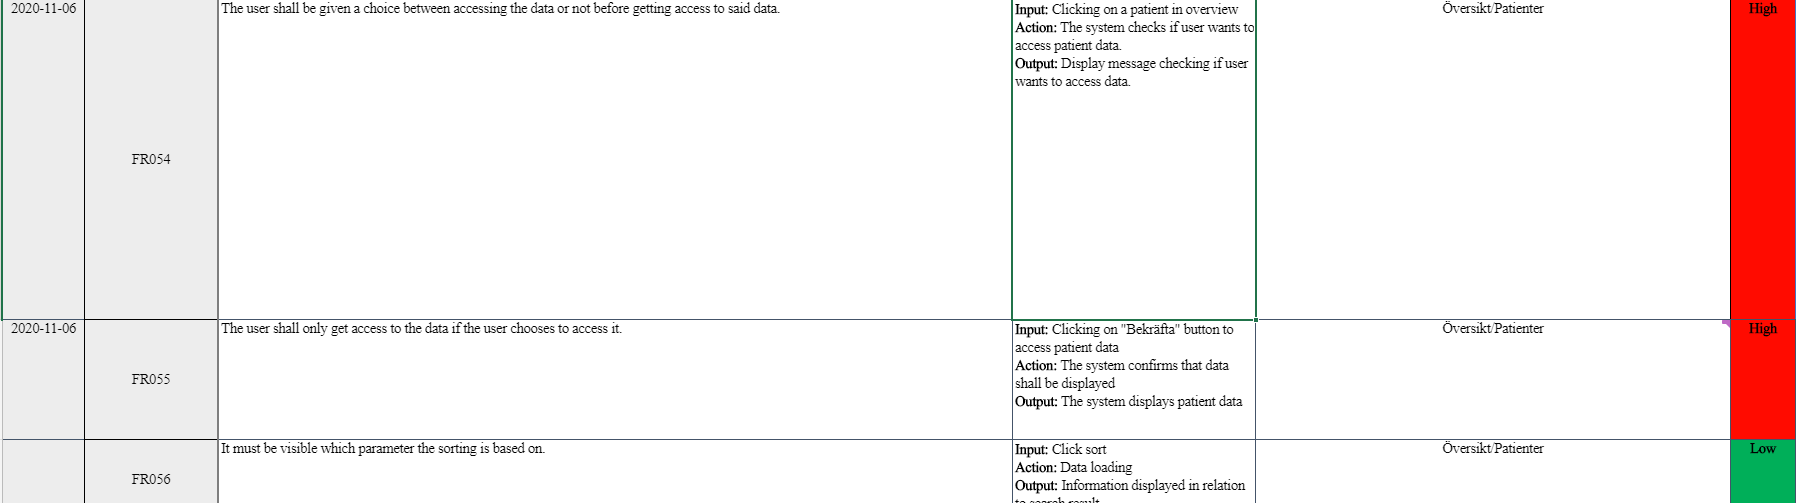
\includegraphics[width=\linewidth]{Pictures/Func8} (8)

    \vfill
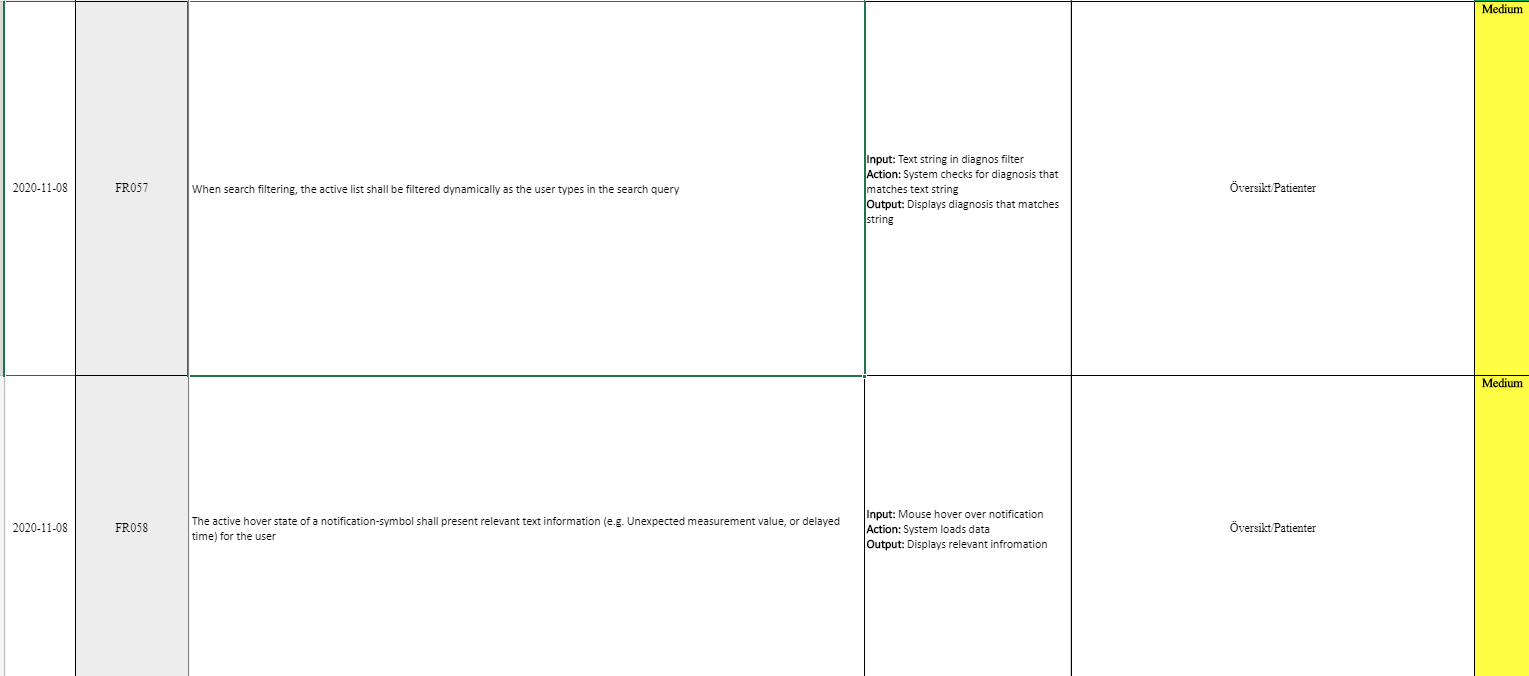
\includegraphics[width=\linewidth]{Pictures/Func9} (9)

    \vfill
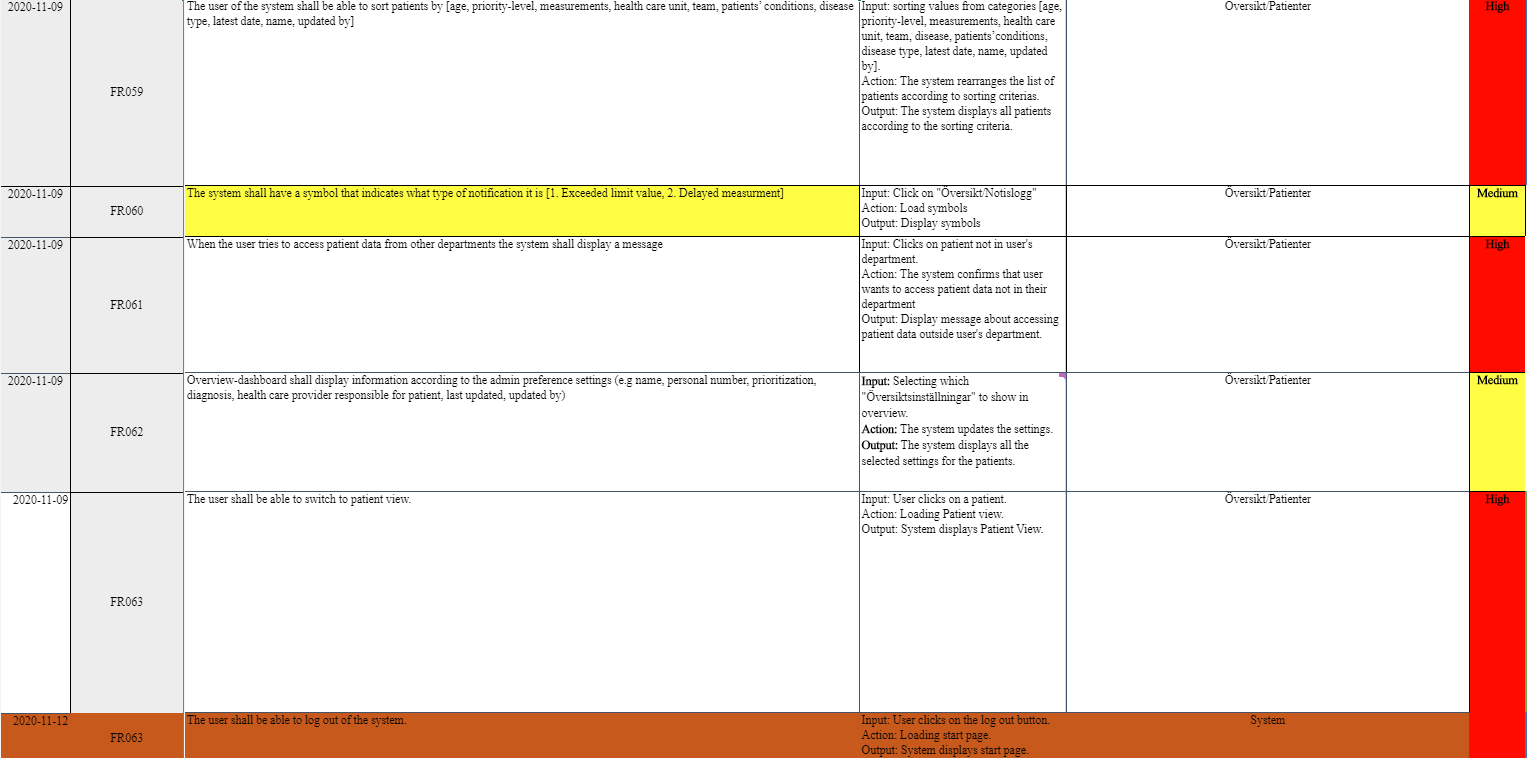
\includegraphics[width=\linewidth]{Pictures/Func10} (10)

    \vfill
\clearpage
\begin{itemize}
    \item Non-Functional Requirements 
\end{itemize}

    \vfill
*Both the Functional and non-functional requirements can be found as larger pictures in Appendix A.
  
  


\subsubsection{Out of Scope (needs more specification)}
Anything outside of our requirements and functionality will not be tested. OpenEHR will only have output tests since we can't manage the DB ourselves. As of 2020/11/11 a big part of unit testing will be scrapped since almost all of our backend functionality comes from OpenEHR, which can't be tested. 
\subsection{Quality Objective}
To ensure that our application will meet the requirements and user tests provided by Region Östergötland. This means both the Functional and non functional requirements. 

To ensure that Bugs and issues are identified using a bug tracking system (TBD) and is continuously checked for bugs.

Using a CI in the Gitlab client to ensure that our code meets the functionality standard set by our automatic tests. By ensuring our CI Heartbyte is looking to implement Continuous Delivery by doing small updates to the software, instead of large feature updates. 
\subsection{Test Logistics}
\subsubsection{Who will test?}
The tests will be made by the Test Leader, Testers and Analysts. Primarily the Test Leader and Tester will make the tests but once the Analysis is done with their tasks, they will join the tests. The tests are then executed.
\subsubsection{When does tests occur?}
The Integration tests will occur once the following input is done:
\begin{itemize}
    \item Software is test ready
    \item A test specification is created
    \item The test Environment is complete
\end{itemize}
Since testing is done in iterations, we will write tests for the parts of the software that is testable, then as software functionality grows, more tests will be added in later iterations. This is also called regression testing.

We will add a couple of integration tests in our CI for the pipeline for the development team, just to quickly check functionality to make sure that functionality is kept at every push of code to the git repository.
\subsection{Roles}
\begin{flushleft}
   \textbf{Test Leader}
    
    
    Gustav Karlsson
  
   \textbf{Tester}
   
    Hjalmar Svensson
    
    Mattis Bark
   
   
   \textbf{Quality Coordinator}
   
    Emma Johansson
     

\end{flushleft}

\subsection{References}
\begin{enumerate}
  \item https://www.guru99.com/test-plan-for-project.html
  \item https://www.ida.liu.se/~TDDC88/theory/07esting.pdf
  \item https://www.udemy.com/course/what-a-java-software-developer-must-know-about-testing/
\end{enumerate}
\clearpage